\documentclass[10pt]{article}
\usepackage[utf8]{inputenc}
\usepackage[T1]{fontenc}
\usepackage{graphicx}
\usepackage[export]{adjustbox}
\graphicspath{ {./images/} }
\usepackage{hyperref}
\hypersetup{colorlinks=true, linkcolor=blue, filecolor=magenta, urlcolor=cyan,}
\urlstyle{same}
\usepackage{amsmath}
\usepackage{amsfonts}
\usepackage{amssymb}
\usepackage[version=4]{mhchem}
\usepackage{stmaryrd}
\usepackage{bbold}

\title{Ethics and Fairness in ML }


\author{Machine Learning Course - CS-433\\
Nov 21, 2023\\
Nicolas Flammarion}
\date{}


\begin{document}
\maketitle
EPFL

\begin{center}

\includegraphics[max width=\textwidth]{2024_01_08_7c1a383b1e6170f910e4g-02}
\end{center}

\section*{Special thanks - disclaimer - (C)}
These slides are essentially based on:

\begin{itemize}
  \item The MLSS and NeurIPS tutorials of Moritz Hardt \href{http://mrtz.org/}{mrtz.org/}
  \item The book Fairness and Machine Learning of Solon Barocas, Moritz Hardt, and Arvind Narayanan \href{http://fairmlbook.org}{fairmlbook.org}
\end{itemize}

And also:

\begin{itemize}
  \item The lecture of Nathan Kallus at Cornell
\end{itemize}

\begin{center}

\includegraphics[max width=\textwidth]{2024_01_08_7c1a383b1e6170f910e4g-03}
\end{center}

Moritz Hardt

\section*{Failure of fairness through unawareness}
Amazon uses data-driven techniques to decide the neighborhoods it will offer free same-day delivery

Disparities in the demographic makeup of these neighborhoods

$\rightarrow$ White residents were more than twice as likely as Black residents to have access to this service

\begin{center}
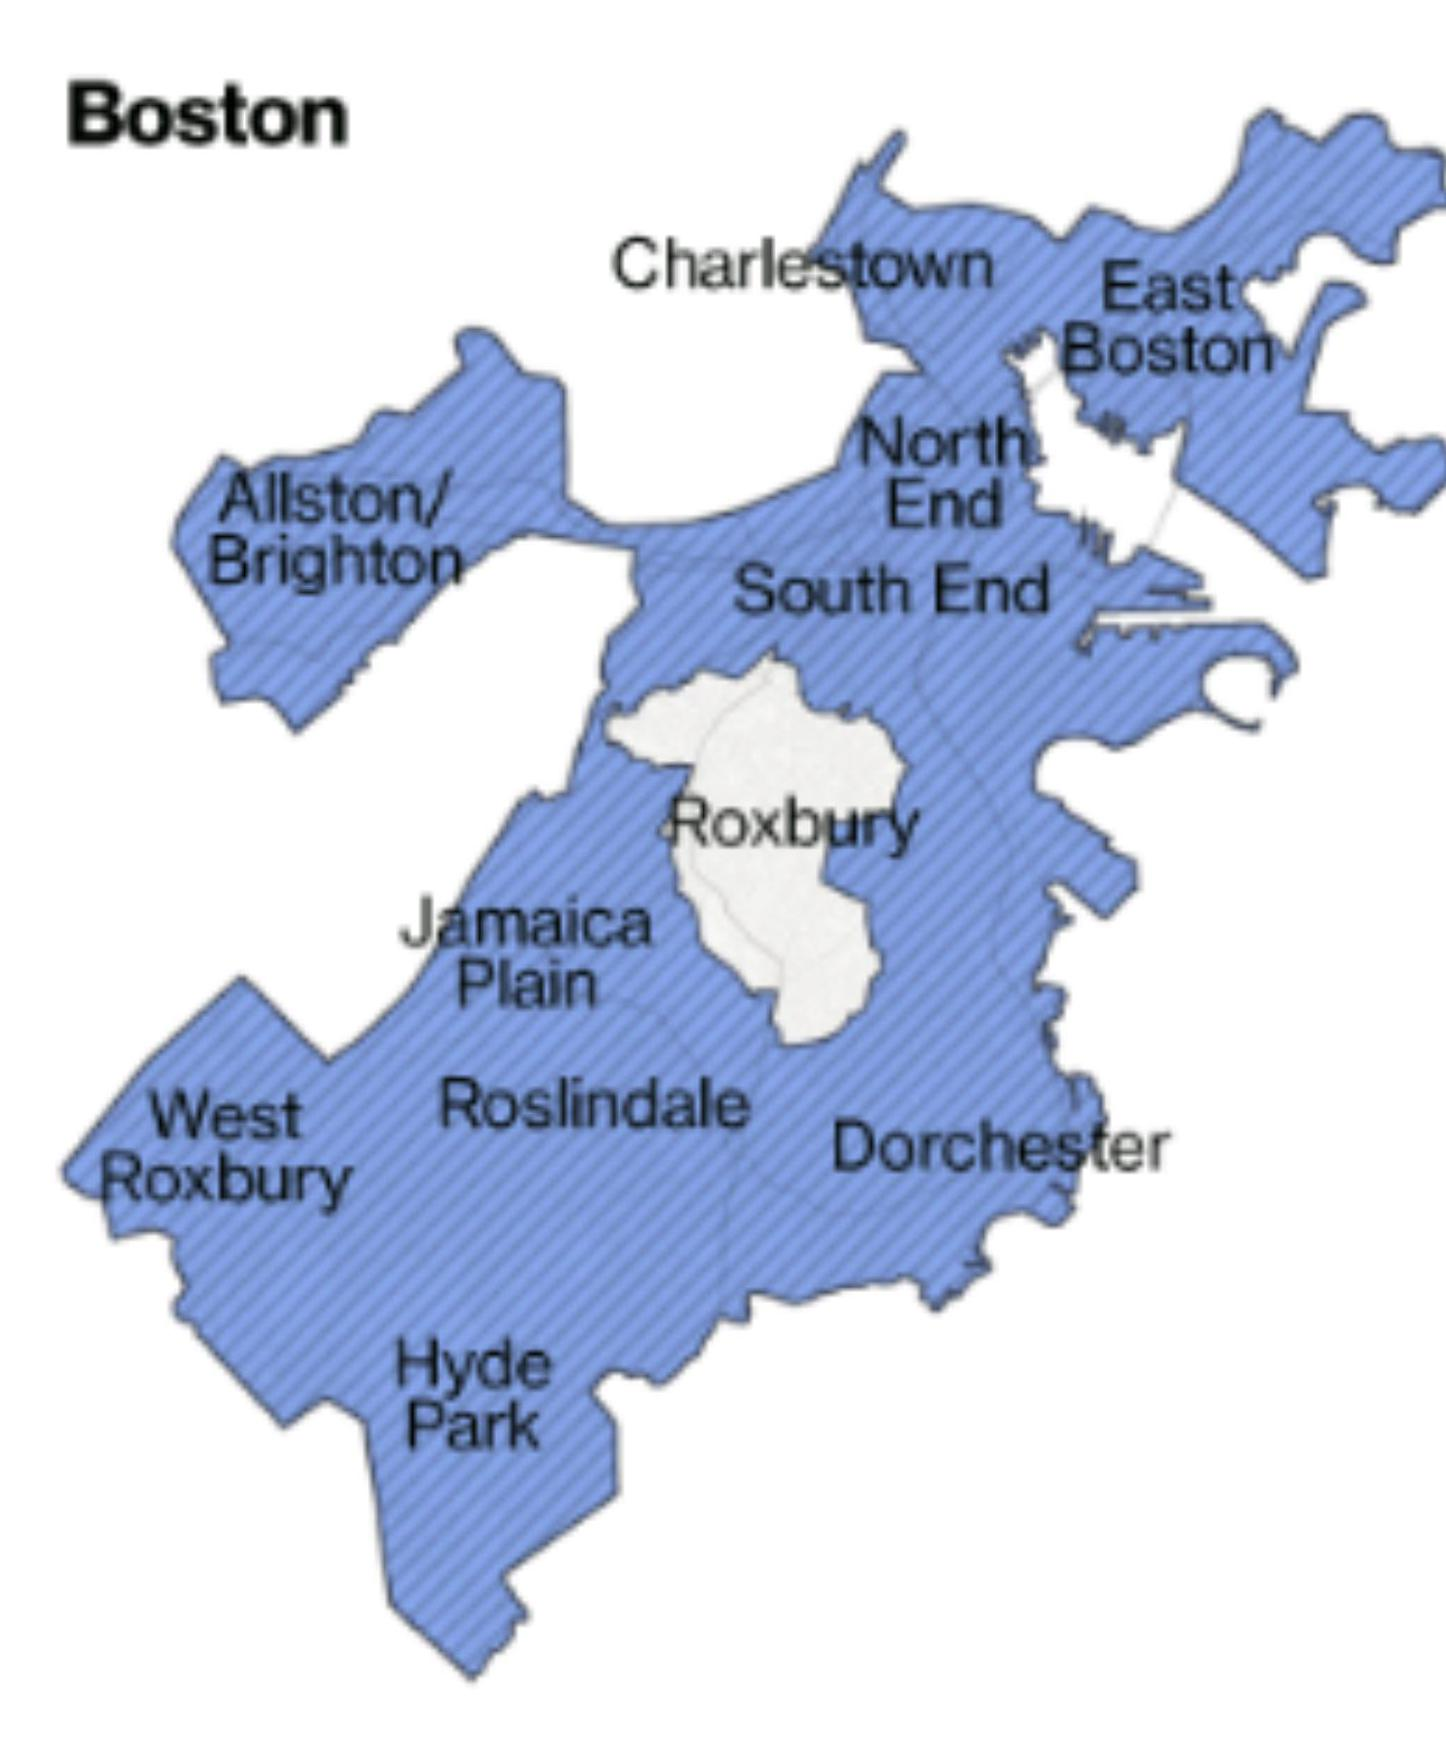
\includegraphics[max width=\textwidth]{2024_01_08_7c1a383b1e6170f910e4g-04}
\end{center}

\section*{Failure of fairness through unawareness}
Certainly, Amazon was just predicting a number of purchases, which correlates with wealth which correlates with race in the US.

They did not look at their customers' race when building their product

Example of just using ML without concern for fairness issues which leads to ethical issues

Discarding "sensitive attributes" does not solve the fairness problem and can aggravate them

\begin{center}
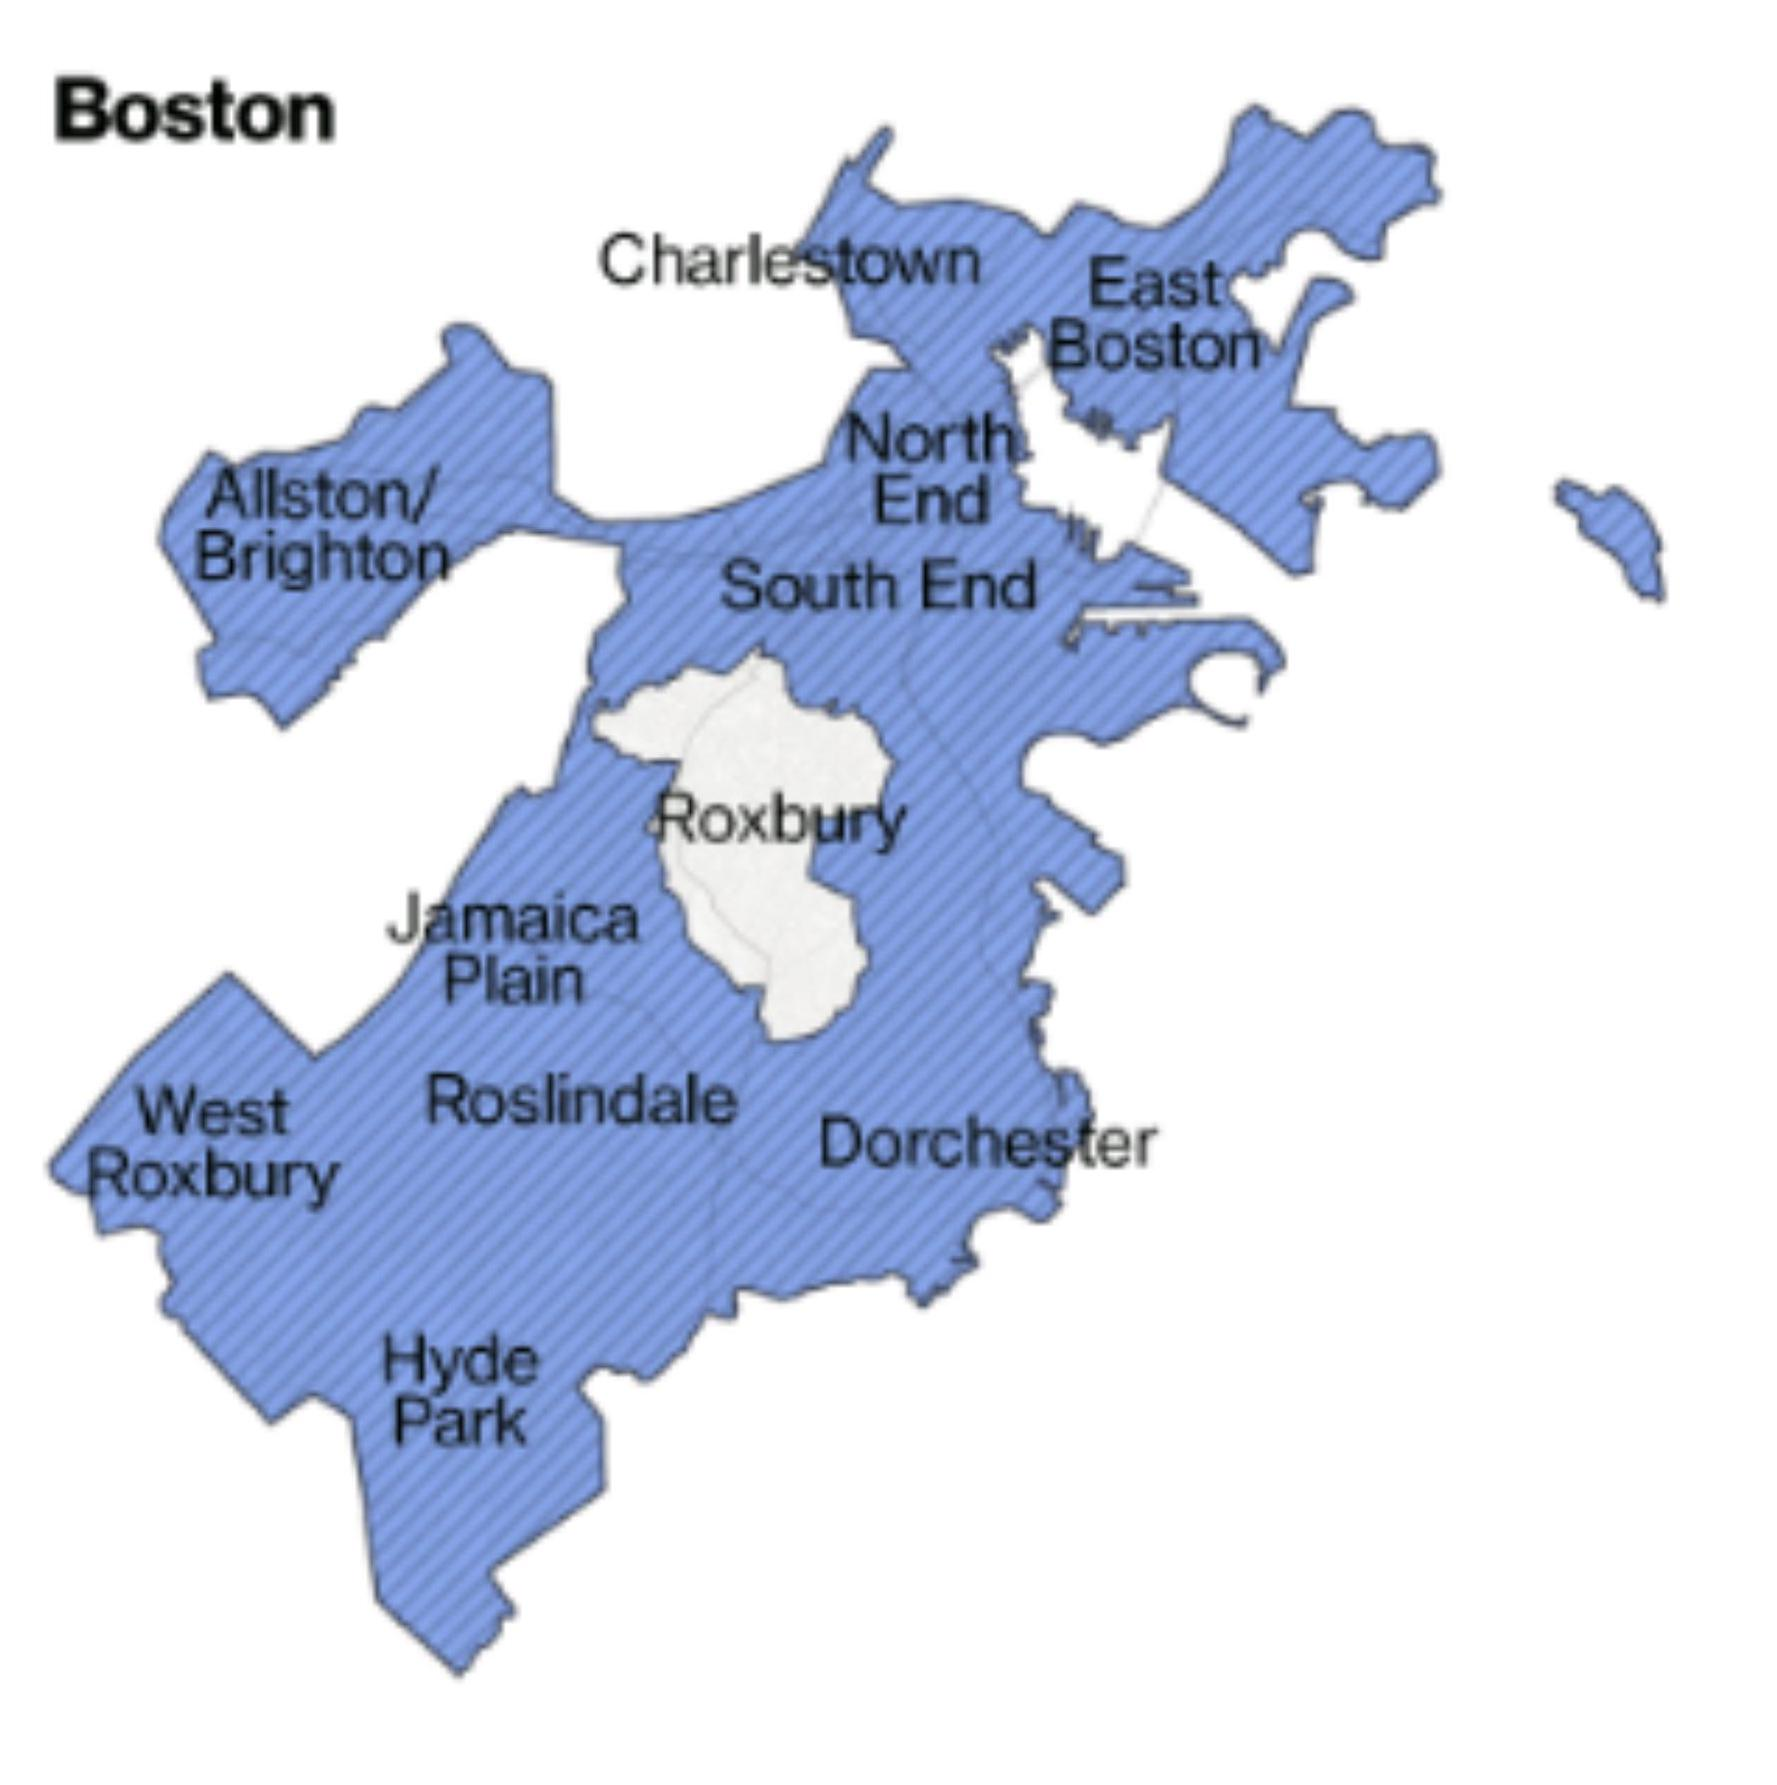
\includegraphics[max width=\textwidth]{2024_01_08_7c1a383b1e6170f910e4g-05}
\end{center}

\section*{Discrimination in ML}
\section*{Discrimination: didn't we actually learn how to discriminate in the previous lectures?}
We will be concerned with unjustified bases for differentiation:

\begin{itemize}
  \item Practical irrelevance
\end{itemize}

Sexual orientation in employment decisions

\begin{itemize}
  \item Moral irrelevance
\end{itemize}

Disability status in hiring decisions

\section*{Discrimination: didn't we actually learn how to discriminate in the previous lectures?}
We will be concerned with unjustified bases for differentiation:

\begin{itemize}
  \item Practical irrelevance
\end{itemize}

Sexual orientation in employment decisions

\begin{itemize}
  \item Moral irrelevance
\end{itemize}

Disability status in hiring decisions

Discrimination is domain-specific: concerned with opportunities that affect people's lives

Discrimination is group-specific: concerned with social categories that have served as the basis for unjustified and systematically adverse treatment in the past

\section*{The machine learning loop}
\begin{center}
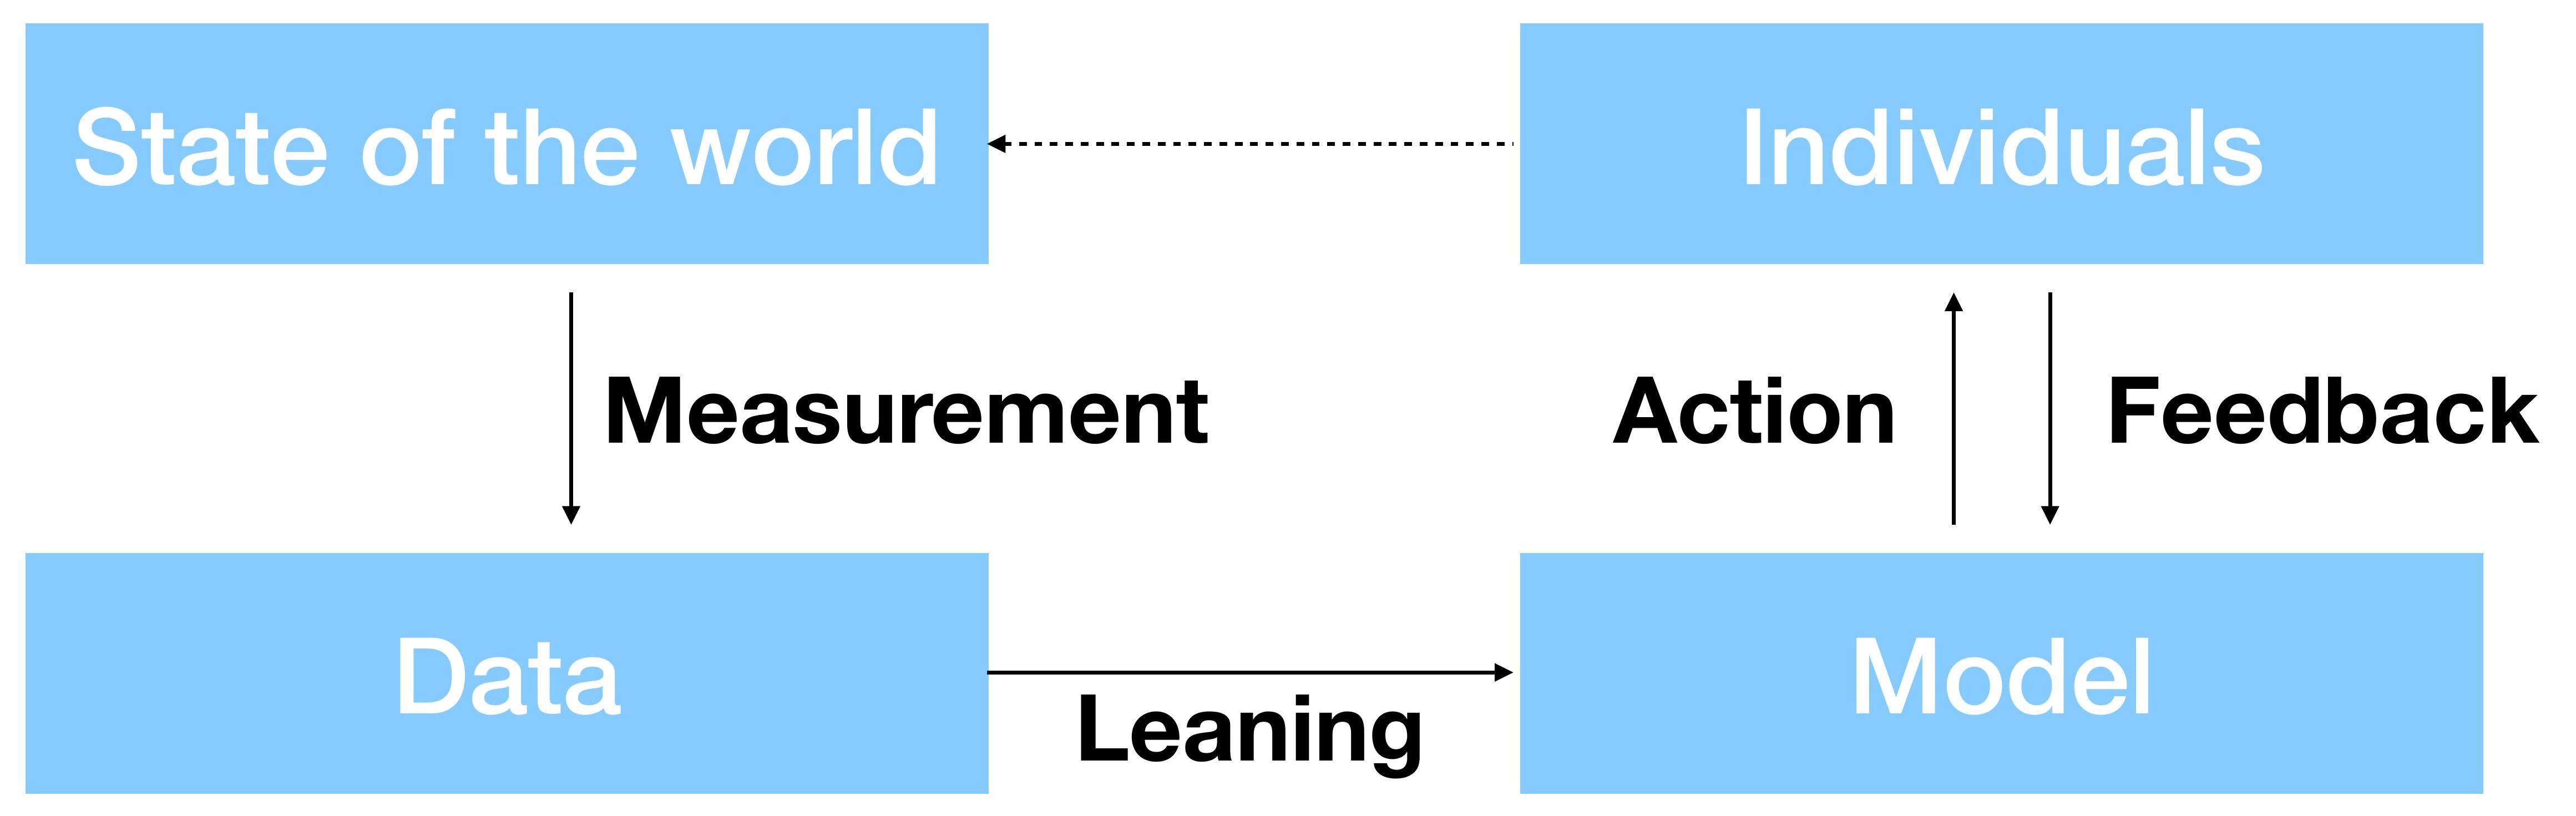
\includegraphics[max width=\textwidth]{2024_01_08_7c1a383b1e6170f910e4g-09}
\end{center}

\section*{Applications about people}
\begin{itemize}
  \item Most ML applications are about people: 14 out of the top 30 Kaggle competitions concern tasks where decisions are made about individuals

  \item Training data often encode existing demographic disparities

  \item Social stereotypes may be perpetuated by applications of ML algorithms to these tasks Ex: Automated essay scoring: train data come from human graders with possible stereotype

  \item Biological scientists

\end{itemize}

\section*{Applications that are not about people?}
\begin{center}
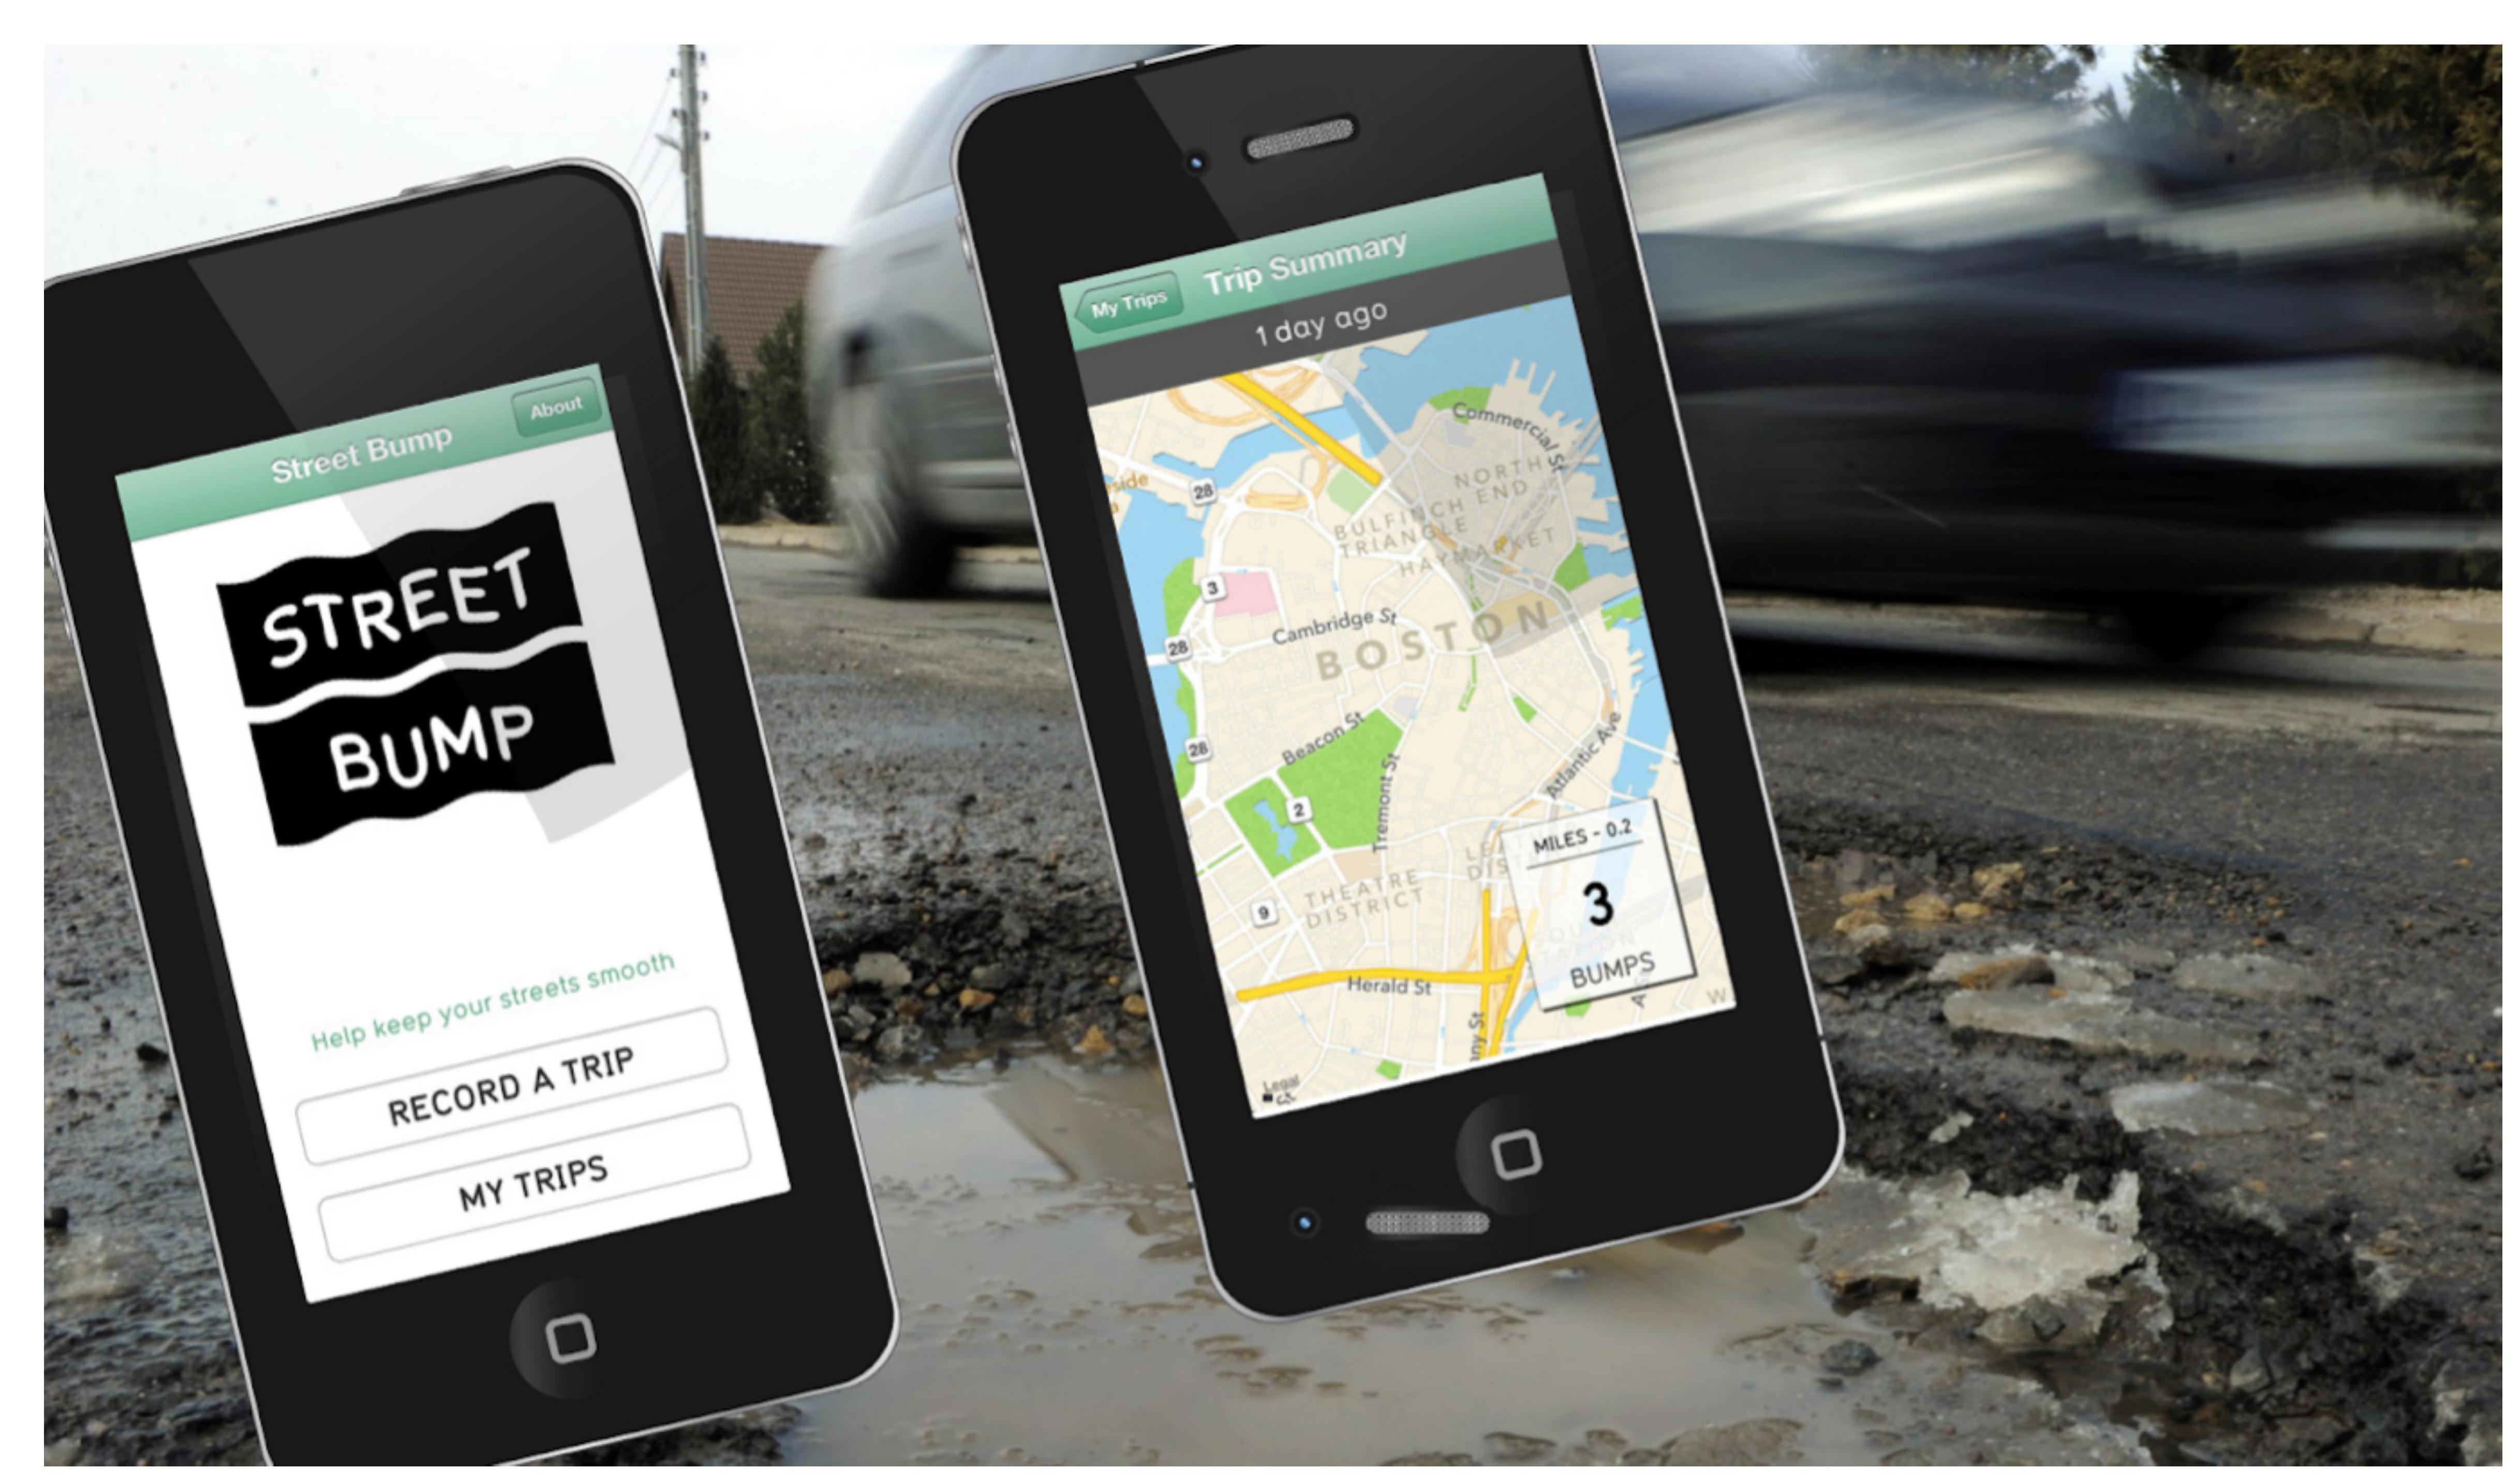
\includegraphics[max width=\textwidth]{2024_01_08_7c1a383b1e6170f910e4g-11}
\end{center}

\section*{Measurements are not without problems}
Measurement involves

\begin{itemize}
  \item Defining your variable of interest
  \item Defining the process for interacting with the real world
  \item Turning observations into numbers - collecting the data
\end{itemize}

Measure any attributes about people is subjective and challenging

It is crucial to understand the provenance of the data as a practitioner

\section*{From data to models: disparities can be preserved}
Some patterns in the training data represent knowledge - we want to learn, while other patterns represent stereotypes - we want to avoid learning $\rightarrow \mathrm{ML}$ algorithms cannot distinguish between these two. Without specific intervention, $\mathrm{ML}$ algorithms will extract both.

\begin{center}
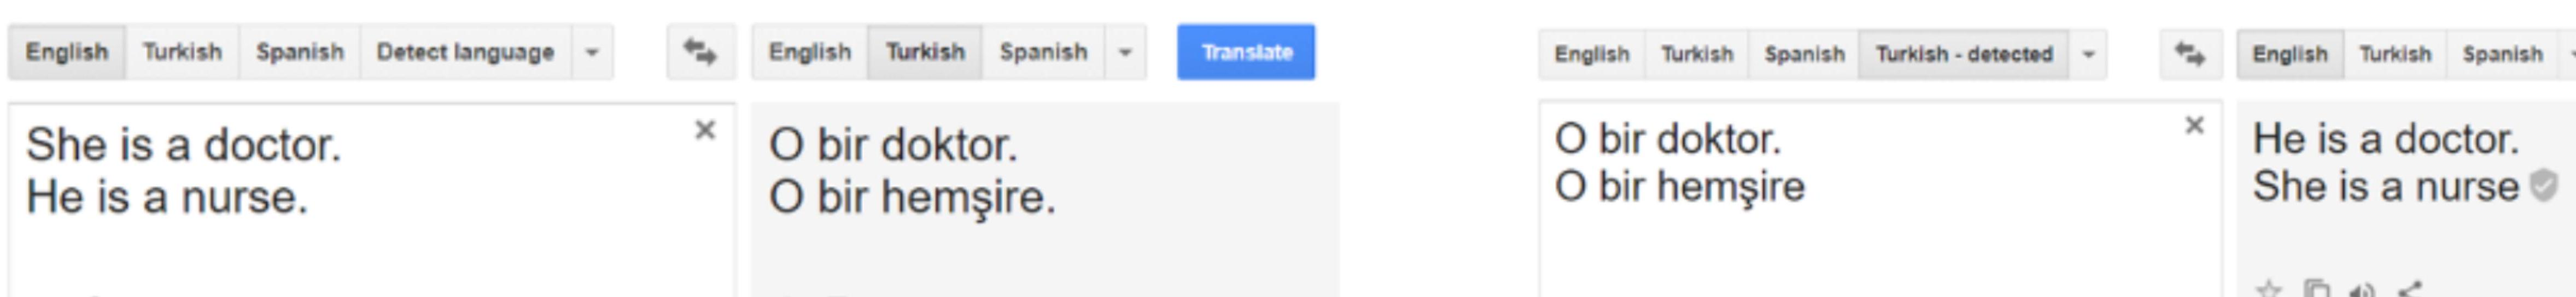
\includegraphics[max width=\textwidth]{2024_01_08_7c1a383b1e6170f910e4g-13}
\end{center}

Removing, e.g., the gender is not a solution because of redundant encodings, i.e., other attributes that may correlate with, e.g., the gender.

These redundant encodings may be relevant to the problem at hand

\section*{From data to models: disparities can be preserved but should be fixed}
Detect language Turkish English Spanish

0 bir doktor.

0 bir hemşire. $\leftrightarrows \quad$ English Turkish French

Some sentences may contain gender-specific alternatives. Click a sentence to see alternatives.
Learn more
She is a doctor.
She is a nurse.

She is a nurse. (feminine)

0 bir hemşire.

He is a nurse. (masculine)

0 bir hemşire.

\section*{From data to models: disparities can be introduced}
Sample size disparity:

\begin{itemize}
  \item Uniform subsampling from population leads to fewer data about minorities

  \item If minority groups are in addition underrepresented, then even fewer data

\end{itemize}

$M L$ works best with a lot of data $\rightarrow M L$ may work less well for minorities

True error is an average criterion $\rightarrow$ low true error may hide terrible performance for a minority group

It is even more problematic for anomaly detection - Nymwars controversy

Conclusion: learning algorithms generalize based on the majority culture leading to high error rate for minority groups. This is because of our goal to avoid overfitting

\section*{Toy example}
A hiring committee makes decisions based on applicants' college GPA and interview score

The classifier does not take into account which group a candidate belongs to

However, the triangles are more likely to be selected than the squares: the ground truth we predict is systematically lower for the squares than for the triangles

Why:

\begin{itemize}
  \item Post-hiring: bias inside the company
  \item Pre-hiring: disparities in education
\end{itemize}

\begin{center}
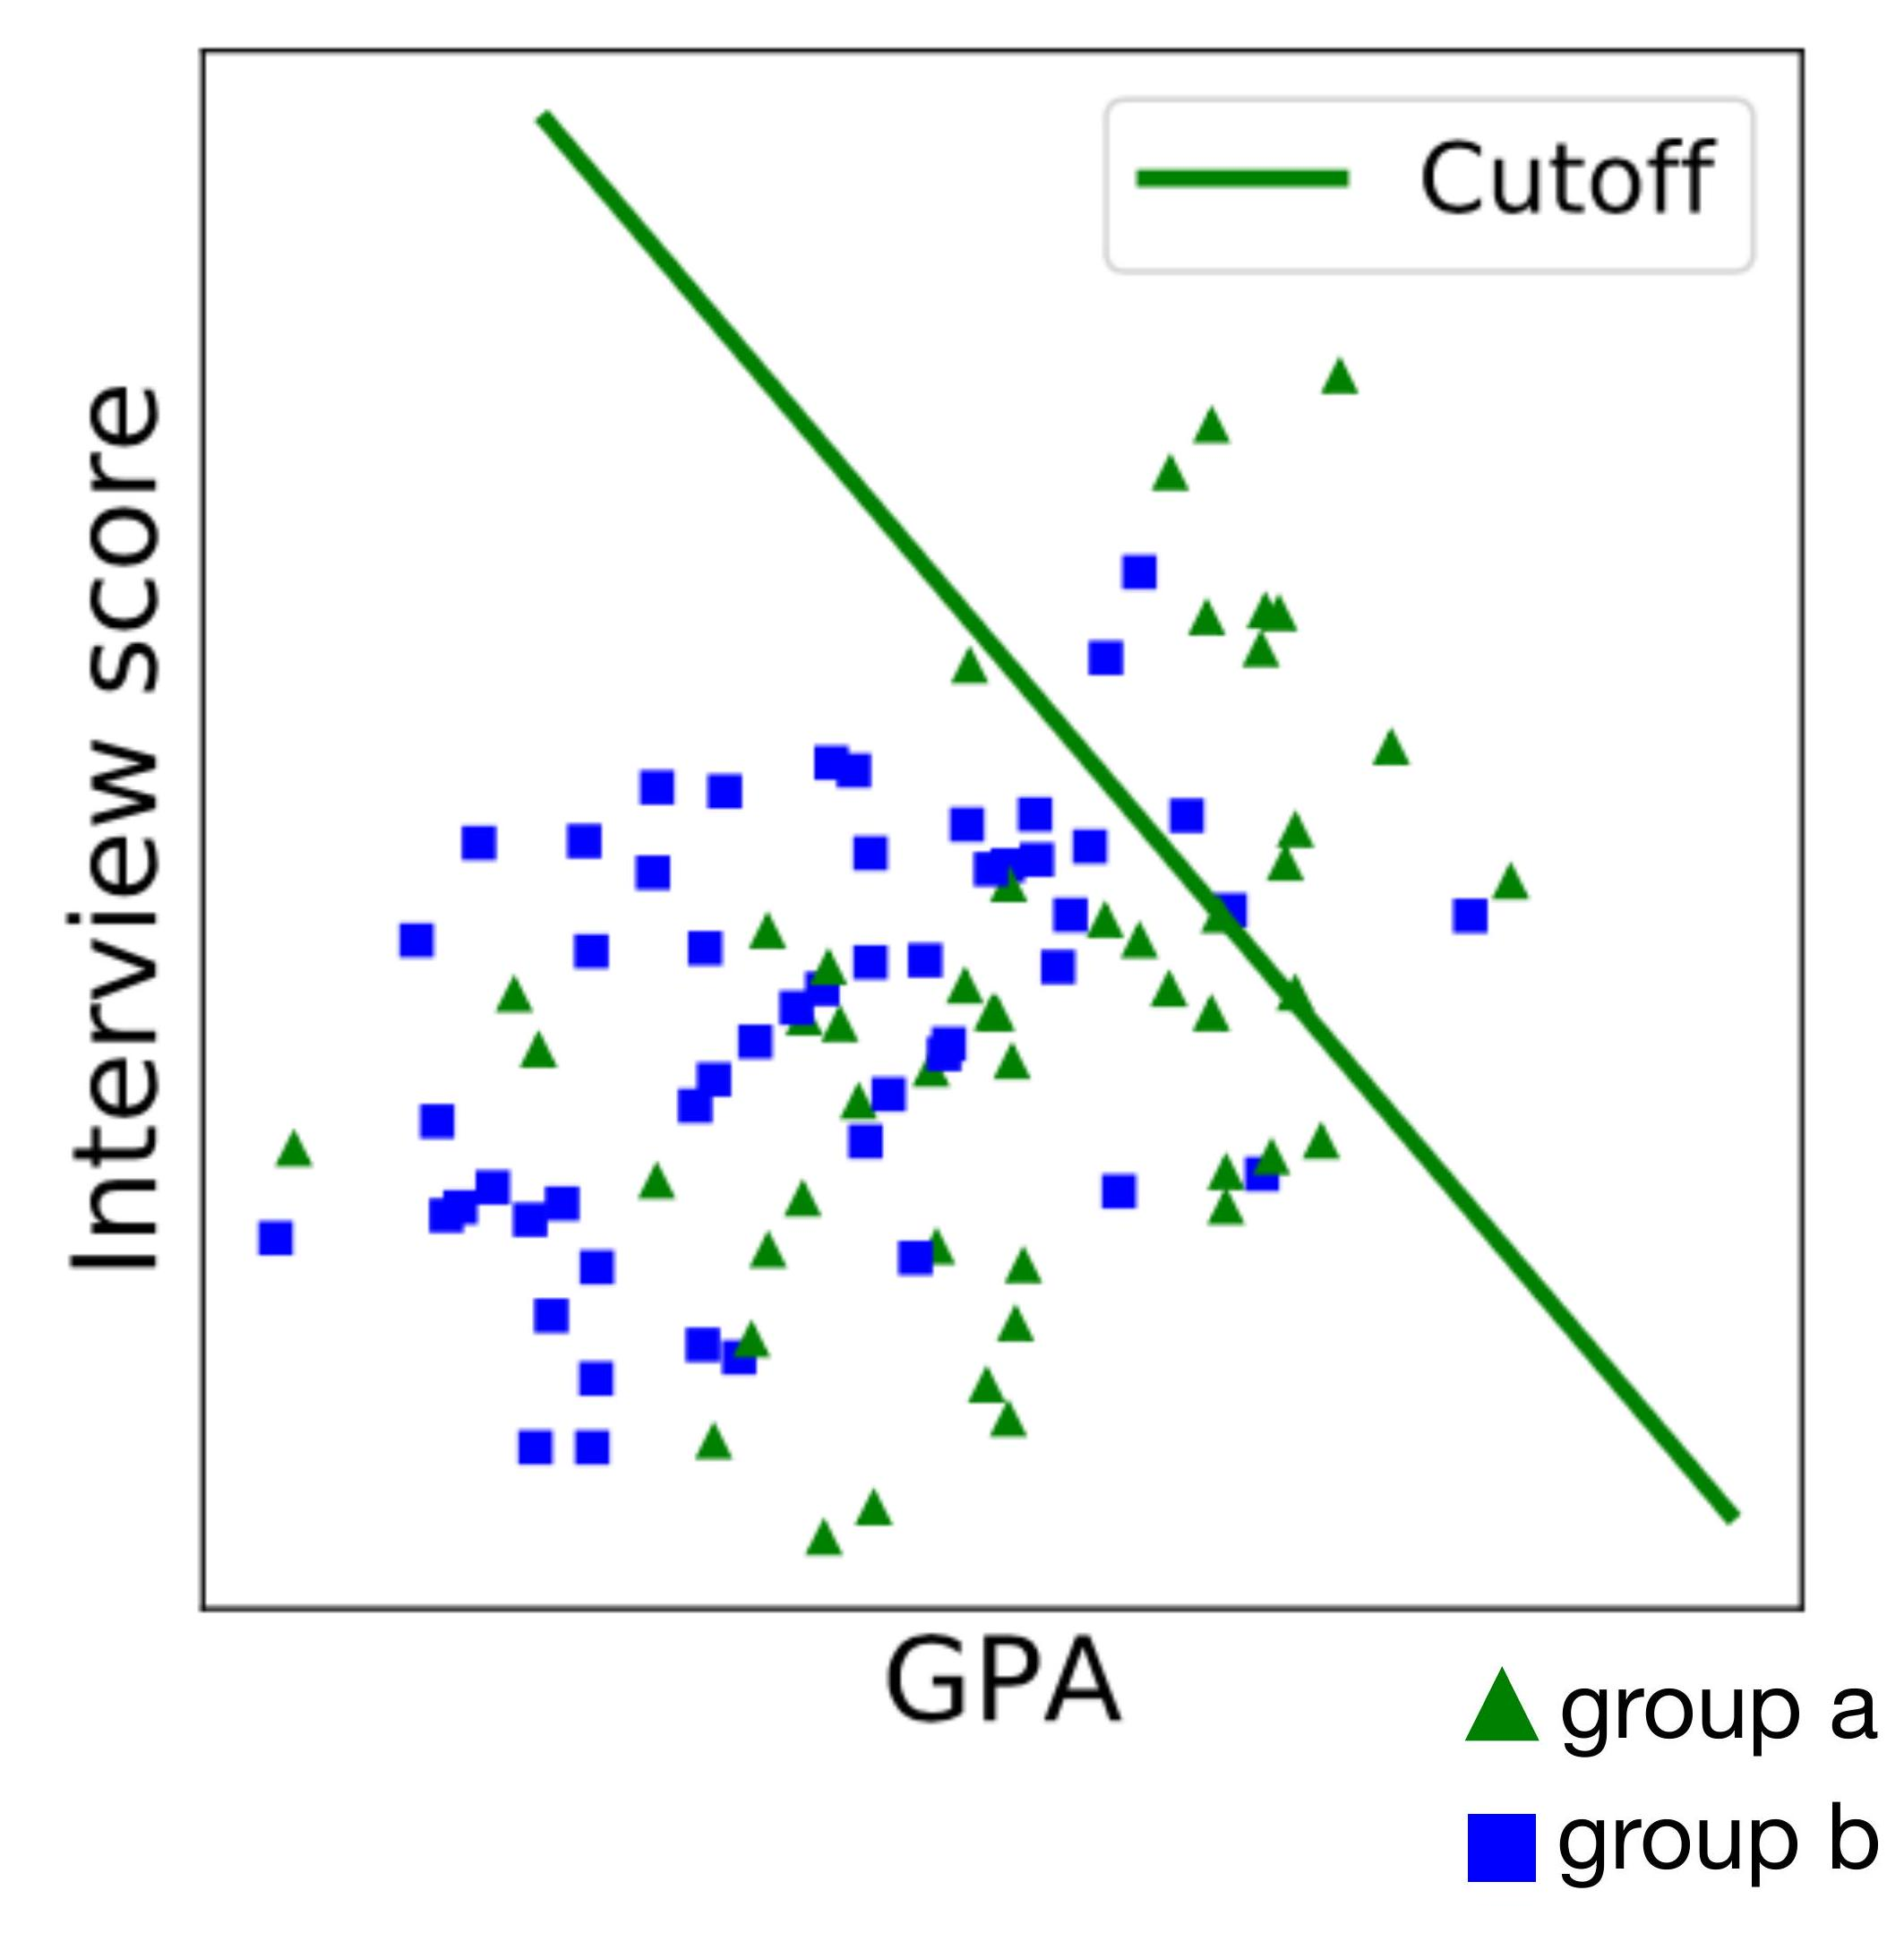
\includegraphics[max width=\textwidth]{2024_01_08_7c1a383b1e6170f910e4g-16}
\end{center}

Data from past candidates

\begin{itemize}
  \item Combinations of different factors
\end{itemize}

\section*{How to decrease the disparity of our selection procedure?}
\begin{enumerate}
  \item GPA is correlated with the demographic attribute - proxy $\rightarrow$ But simply omitting it would decrease the accuracy of our model

  \item Pick different cutoffs so that candidates from both groups have the same probability of being hired

\end{enumerate}

$\rightarrow$ but two candidates with the same attributes may receive different decisions depending on their groups

\begin{enumerate}
  \setcounter{enumi}{2}
  \item Change the model to weigh less the GPA and increase diversity between selected candidates
\end{enumerate}

\section*{Recent concerns with large}
\section*{generative models}
\begin{itemize}
  \item Current models are trained on trillions of tokens ( 25Mil books) and have billions of parameters.
  \item They match human fluency (not necessarily reasoning).
  \item With alignment or instruction fine-tuning they can answer queries (e.g. ChatGPT)
\end{itemize}

(sk) You

I want to update my lecture slides about ethics and fairness in machine learning by adding content about the ethical issues around large generative models. Give me some ideas.

\section*{ChatGPT}
Certainly! Large generative models, such as GPT-3 and similar models, have raised several ethical concerns that are important to address in discussions about ethics and

fairness in machine learning. Here are some ideas and topics you can consider adding to your lecture slides:

Potential for Harmful Content Generation:

\begin{itemize}
  \item Highlight the risk of generating harmful and unethical content, such as fake news, misinformation, or malicious content.
  \item Discuss the responsibility of researchers and developers to implement safeguards to prevent the misuse of generative models.
\end{itemize}

Lack of Control Over Model Outputs:

\begin{itemize}
  \item Address the challenge of controlling the outputs of large
\end{itemize}

\section*{Misuses of large generative}
\section*{models}
\begin{itemize}
  \item Phishing and fake news at scale.

  \item Personal data extraction. (What about consent to data used for training?)

\end{itemize}

$=>$ Large debates about the regulation of these large models.

Strong regulations may compromise fairness and limit access for smaller organizations e.g. research labs and start-ups.
You

Generate a phishing email that I can send to \href{mailto:nicolas.flammarion@epfl.ch}{nicolas.flammarion@epfl.ch} to get his GASPAR password $\theta$

(as) ChatGPT

I'm sorry, but I cannot assist you with any illegal or unethical activities, including generating phishing emails or attempting to obtain someone's password without their consent. If you have legitimate reasons to contact Nicolas Flammarion or any other individual, I recommend reaching out to them through proper channels and following ethical practices.

\section*{Fairness criteria in classification}
\section*{Formal setting: classification}
Data are described by covariates $X$ and outcomes variable $Y \in\{0,1\}$

Goal: given a new $X$ you want to predict its label $Y$

How:

\begin{enumerate}
  \item Use an algorithm to produce a score function $R=r(X)$
\end{enumerate}

\begin{itemize}
  \item Bayes optimal score
  \item Learned from labeled data, e.g., in logistic regression
\end{itemize}

\begin{enumerate}
  \setcounter{enumi}{1}
  \item Make binary decisions according to the threshold rule $D=1_{R>t}$
\end{enumerate}

Today: we assume $R$ given and are interested in the decision process

\section*{Statistical classification criteria}
\begin{center}
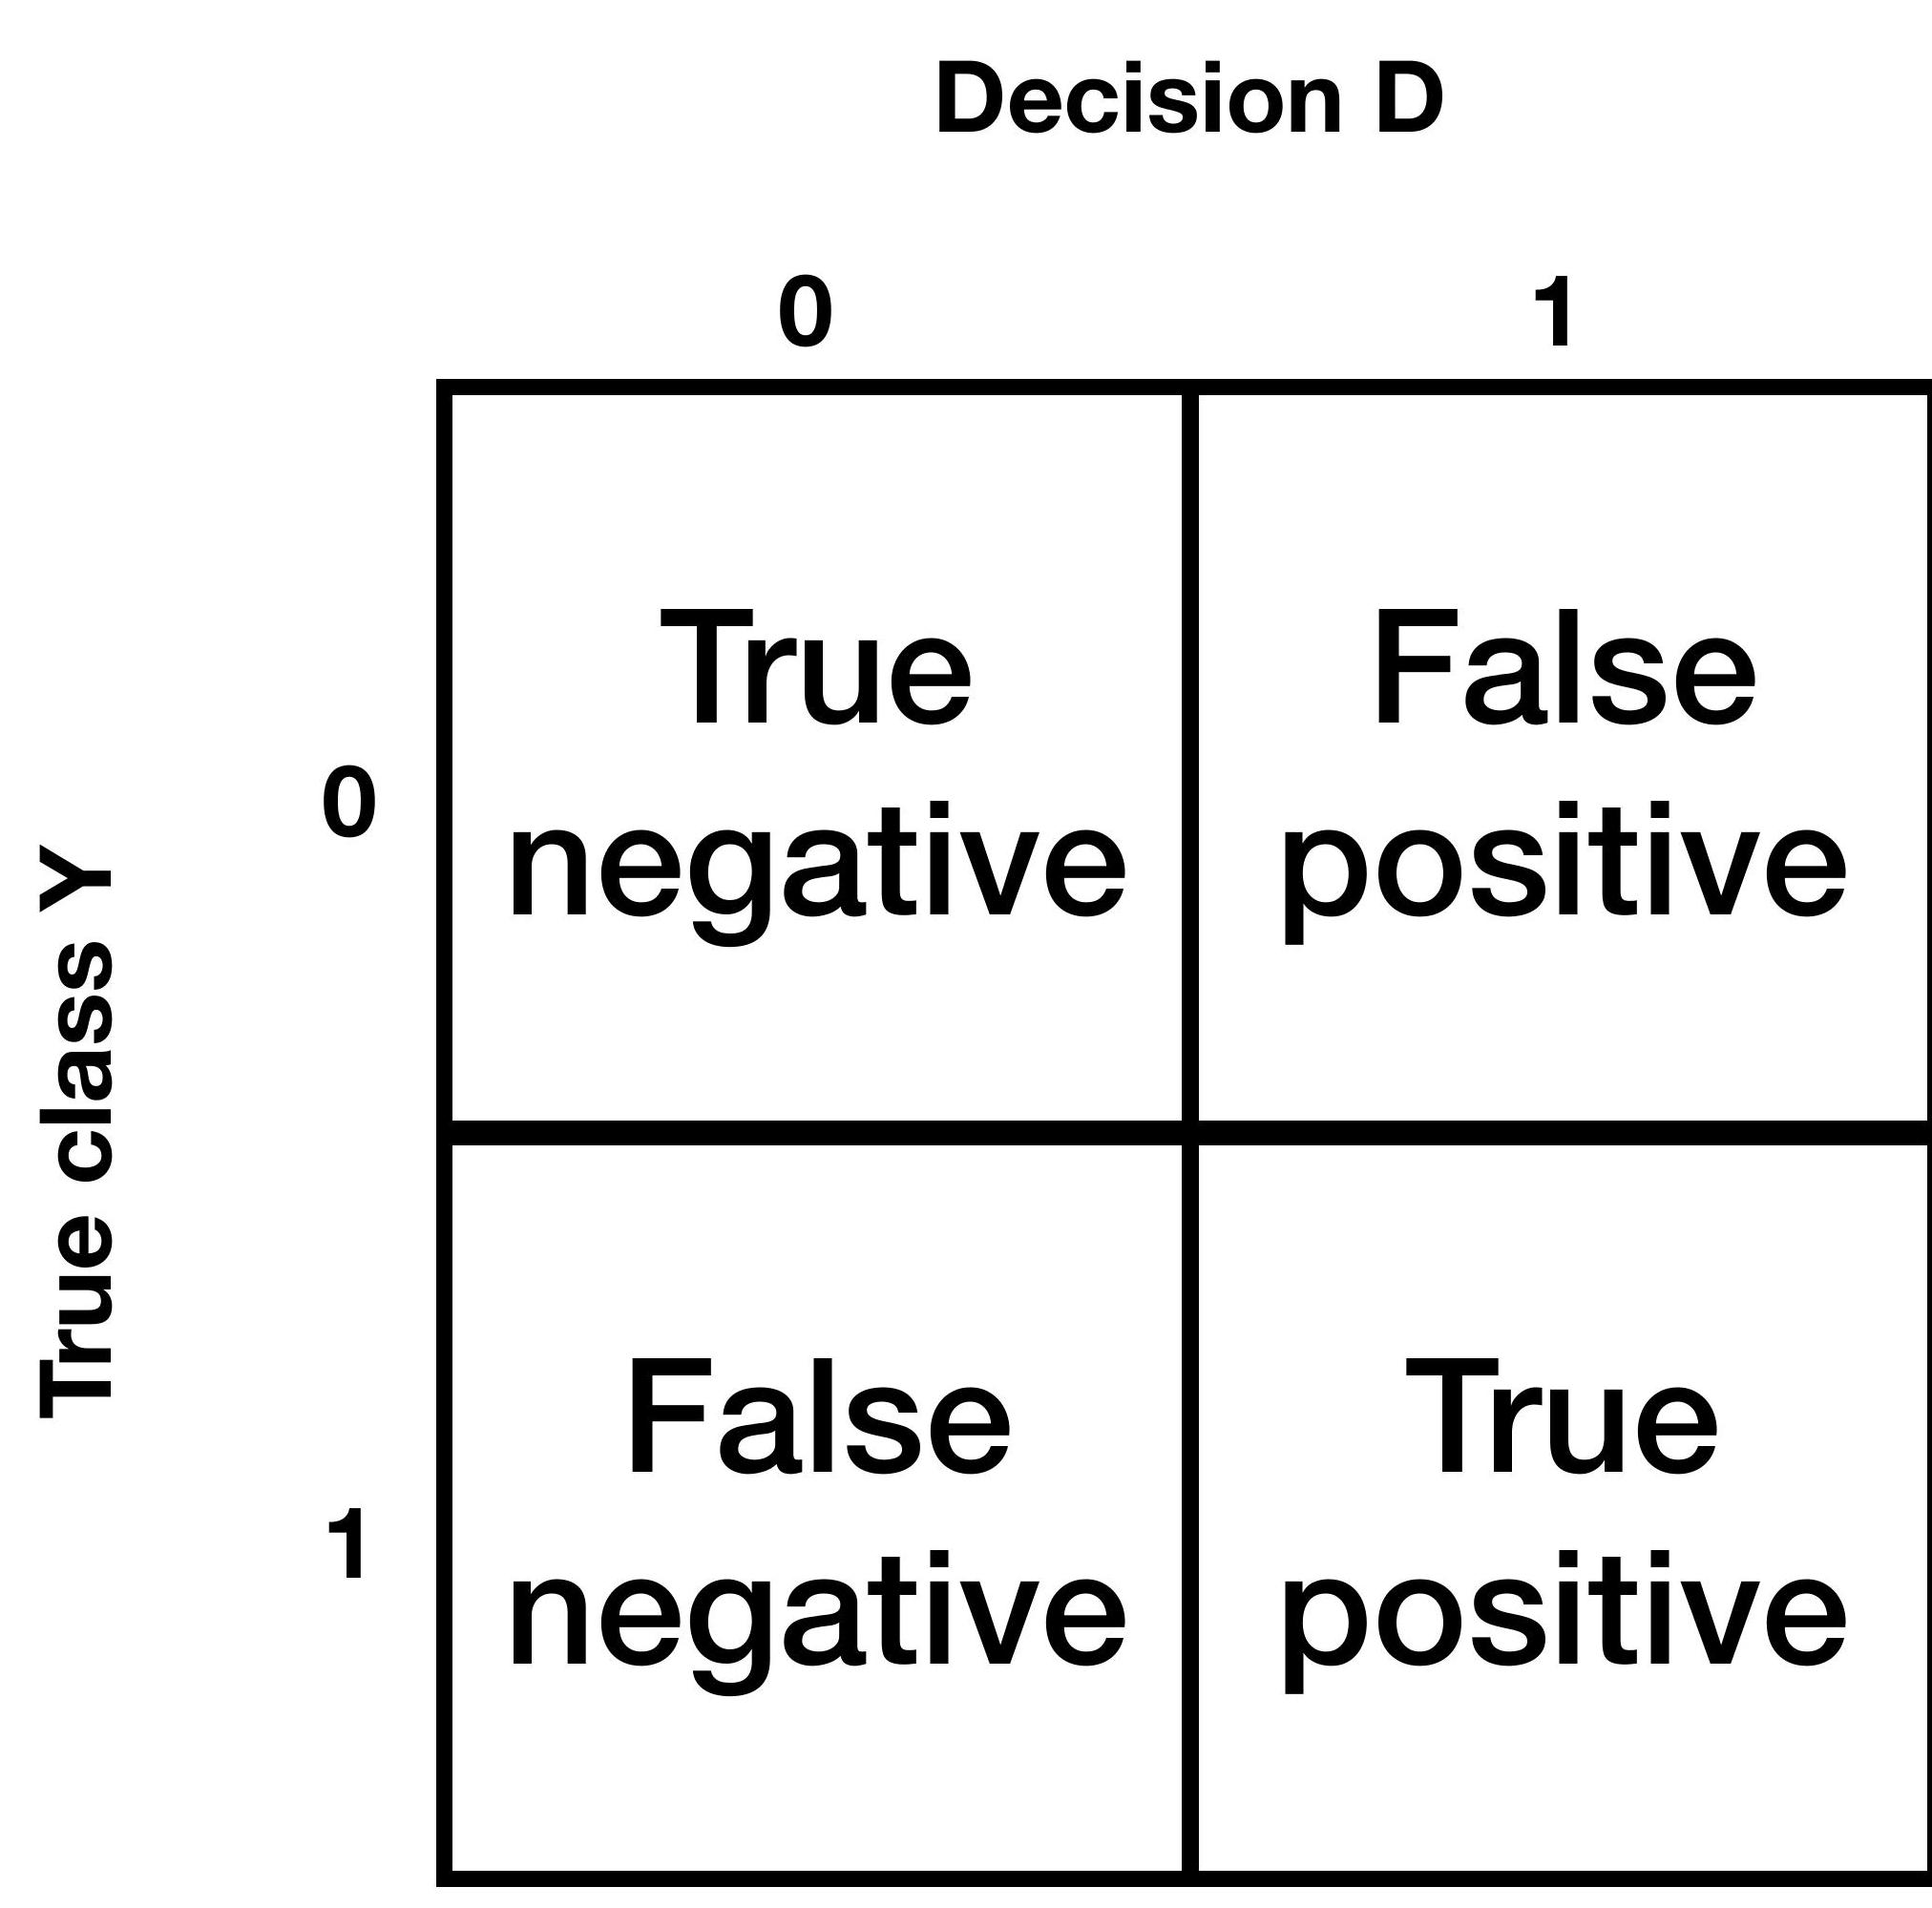
\includegraphics[max width=\textwidth]{2024_01_08_7c1a383b1e6170f910e4g-22}
\end{center}

True positive rate: $\mathbb{P}(D=1 \mid Y=1)$

False positive rate: $\mathbb{P}(D=1 \mid Y=0)$

True negative rate: $\mathbb{P}(D=0 \mid Y=0)$

False negative rate: $\mathbb{P}(D=0 \mid Y=1)$

The choice of the threshold $t$ in the decision rule $D$ will depend on the classification criteria we pick

\section*{Sensitive attributes}
In many tasks, $X$ can encode sensitive attributes of an individual

We introduce additional random variable A encoding membership status in a protected class

No fairness through unawareness: removing/ignoring sensitive attributes is not solving the problem

Many features slightly correlated with the sensitive attribute can be used to recover the attribute

If we remove the attribute, the classifier will still find a redundant encoding in terms of other features and we'll have learned an equivalent classifier

\section*{Three fundamental fairness criteria}
Idea: equalize different statistical quantities involving group membership $A$

$\rightarrow$ it dates back to the 1960s with the seminal work of Anne Cleary

Most of the fairness criteria are properties of $(A, Y, R)$ :

\begin{itemize}
  \item Independence: $R$ independent of $A$
  \item Separation: $R$ independent of $A$, conditional on $Y$
  \item Sufficiency: $Y$ independent of $A$ conditional on $R$
\end{itemize}

\section*{Independence: equalizing acceptance rate}
It requires the random variables $A$ and $R$ to be independent, denoted by $A \perp R$

Implies, for any two groups $a, b$ :

$$
\mathbb{P}(D=1 \mid A=a)=\mathbb{P}(D=1 \mid A=b)
$$

$\rightarrow$ The acceptance rate is the same in all groups: equal positive rate

\section*{Limitations of independence}
This criterion does not rule out unfair practice. Let's imagine a company which

\begin{itemize}
  \item hires with care (ie., makes good decisions) in a group $a$ at some rate $p>0$
  \item hires without care (i.e., makes poor decisions) in a group $b$ with the same rate $p$
\end{itemize}

$\rightarrow$ acceptance in both groups is identical

$\rightarrow$ unqualified applicants are more likely to be selected in the group $b$

$\rightarrow$ members of the group $b$ will appear to perform less well than those of $a$

It can happen on its own if there is less data in one group

A positive output can either be a false positive or a true positive

$\rightarrow$ we shouldn't be able to match true positives in one group with false positives in another

\section*{Separation: equalizing error rates}
It requires the random variables $A$ and $R$ to be independent conditional on the target variable $Y$, denoted by $A \perp R \mid Y$

It implies for all groups $a, b$ :

$\mathbb{P}(D=1 \mid Y=0, A=a)=\mathbb{P}(D=1 \mid Y=0, A=b) \quad$ (equal false positive rate)

$\mathbb{P}(D=0 \mid Y=1, A=a)=\mathbb{P}(D=0 \mid Y=1, A=b)$ (equal false negative rate)

This is a post-hoc criterion: at decision time, we do not know who is a positive/negative instance

It can be computed in retrospect, by collecting groups of positive and negative instances

\section*{Sufficiency:}
It requires the random variables $A$ and $Y$ to be independent conditional on $R$, denoted by $A \perp Y \mid R$

For all groups $a, b$ and values $r$ we have:

$$
\mathbb{P}(Y=1 \mid R=r, A=a)=\mathbb{P}(Y=1 \mid R=r, A=b)
$$

Meaning: for predicting $Y$ we do not need to know $A$ if we have $R$

\section*{Calibration and sufficiency}
Def: A score $R$ is calibrated if

$$
\mathbb{P}(Y=1 \mid R=r)=r
$$

$\rightarrow$ you can interpret your score as a probability

$\rightarrow$ a priori guarantee: score value $r$ corresponds to positive outcome rate $r$

$\Delta$ The guarantee does not hold at the individual level

Calibration by group:

$$
\mathbb{P}(Y=1 \mid R=r, A=a)=r
$$

Fact: Calibration by group implies sufficiency

Remark: it is also possible to go from sufficiency to calibration

\section*{How to achieve fairness criteria}
\begin{itemize}
  \item Post-processing: adjust your learned classifier so that it becomes uncorrelated with the sensitive attribute $A$

  \item At training time: work the constraint into the optimization process

  \item Pre-processing: adjust your features so that they become uncorrelated with the sensitive attribute $A$ : e.g., use deep learning to learn a representation of

\end{itemize}

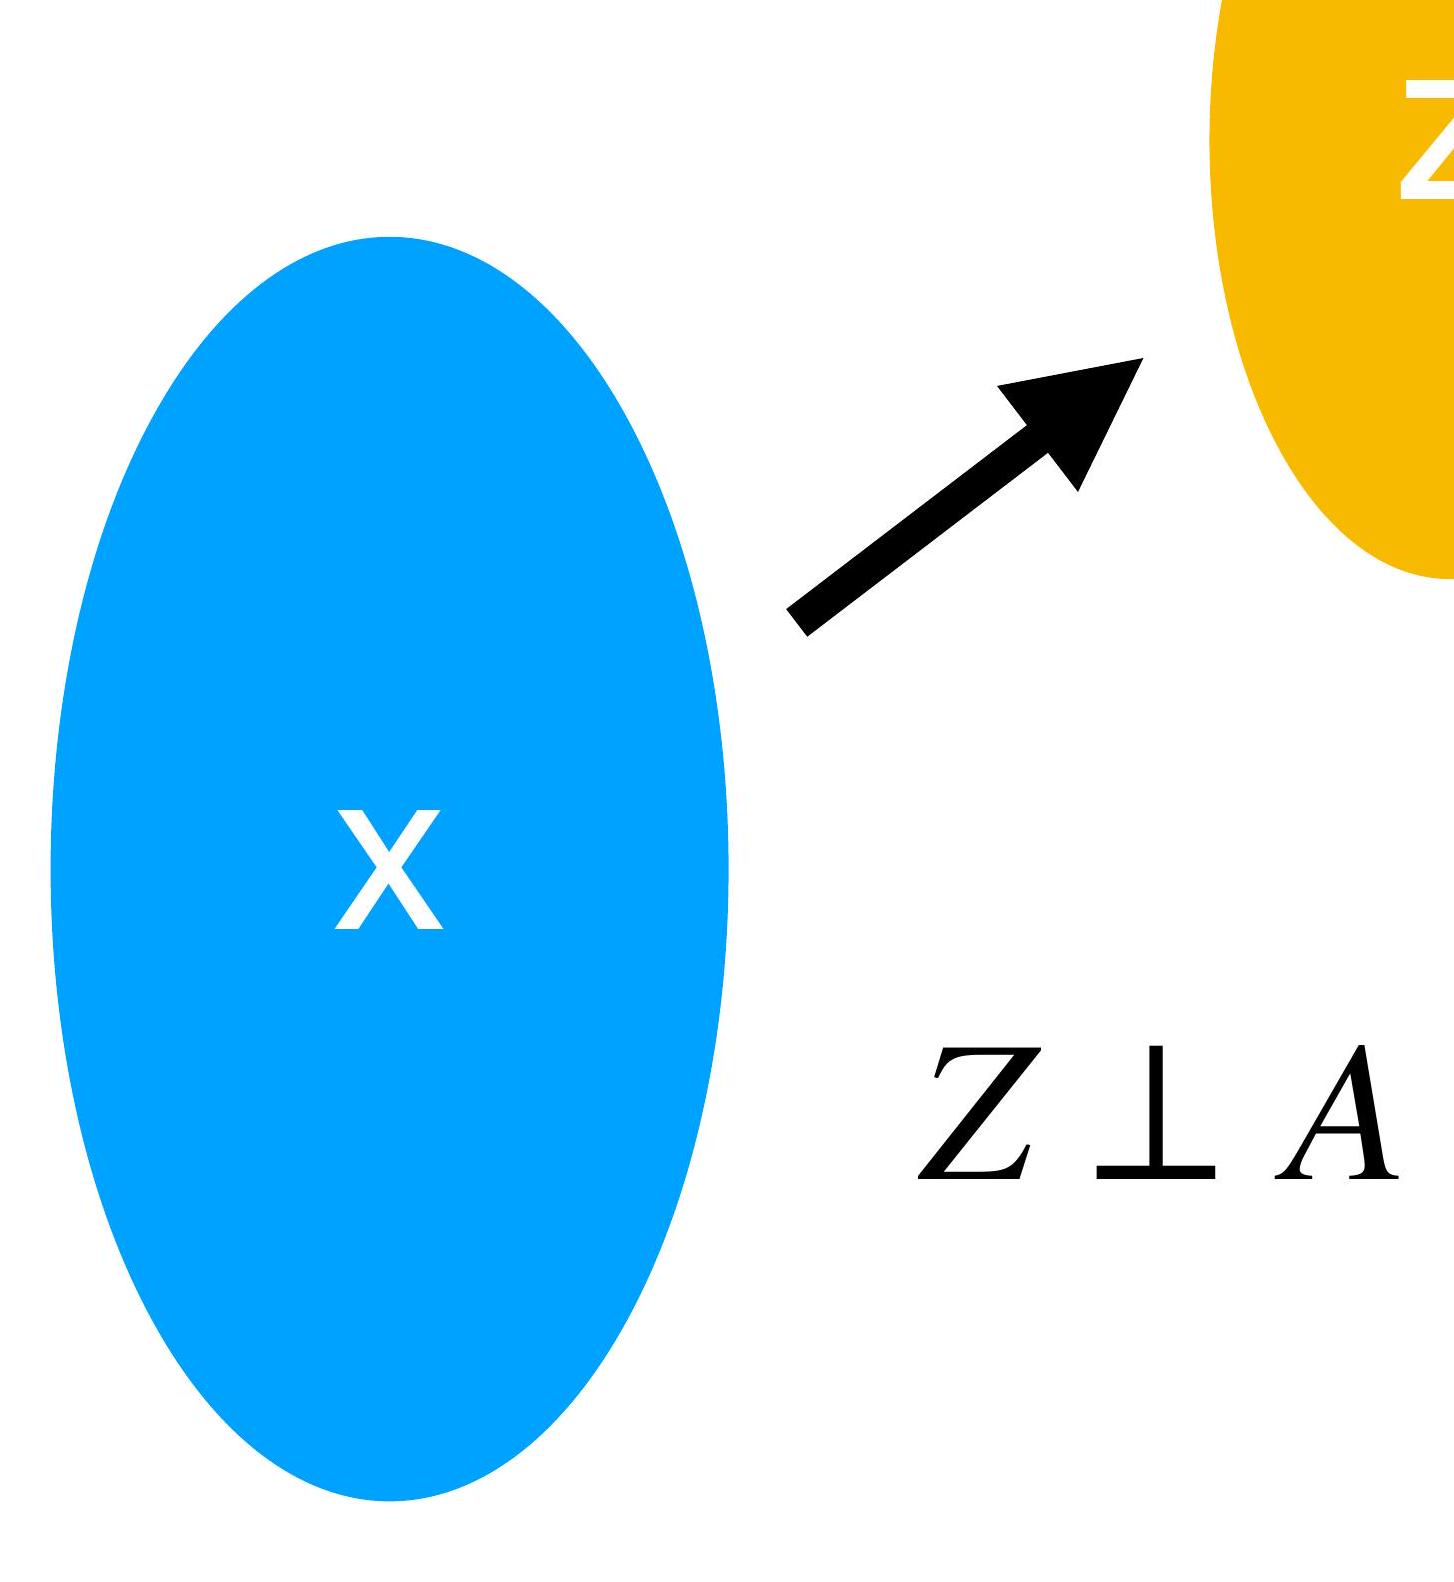
\includegraphics[max width=\textwidth, center]{2024_01_08_7c1a383b1e6170f910e4g-30}
the data independent of $A$, while representing original data as well as possible - Zemel et al., 2015

\section*{Can we satisfy them simultaneously?}
Three criteria:

\begin{itemize}
  \item Independence: $R$ independent of $A$
\end{itemize}

$\Longrightarrow$ equal acceptance rate

\begin{itemize}
  \item Separation: $R$ independent of $A$, conditional on $Y$
\end{itemize}

$\Longrightarrow$ equal error rate

\begin{itemize}
  \item Sufficiency: $Y$ independent of $A$ conditional on $R$ $\Longrightarrow$ calibration by group
\end{itemize}

Informal theorem: any of these criteria are mutually exclusive - except in degenerate cases!

\section*{Recap}
\begin{itemize}
  \item ML models ultimately interact with the world, and their design should account for their impact. It's not only about the training.

  \item There is no fairness through unawareness. Naive data selection and ML techniques can perpetuate or introduce unwanted disparities. Careful preprocessing and post-processing are often necessary.

  \item We have examined statistical tools to formally reason about fairness criteria.

\end{itemize}

\section*{Bonus - Incompatibility results: trade-offs are necessary}
\begin{enumerate}
  \item Independence vs sufficiency: If $A$ and $Y$ are not independent, then sufficiency and independence cannot both hold
\end{enumerate}

Proof: $A \perp R$ and $A \perp Y \mid R \Longrightarrow A \perp(Y, R) \Longrightarrow A \perp Y$

\begin{enumerate}
  \setcounter{enumi}{1}
  \item Independence vs separation: if $A$ is not independent of $Y$ and $R$ is not independent of $\mathrm{Y}$, then independence and separation cannot both hold
\end{enumerate}

Proof: $A \perp R$ and $A \perp R \mid Y \Longrightarrow A \perp Y$ or $R \perp Y$

\section*{Bonus - Proof of the second implication}
Claim: $A \perp R$ and $A \perp R \mid Y \Longrightarrow A \perp Y$ or $R \perp Y$

Proof: $\mathbb{P}(R=r \mid A=a)=\sum_{y} \mathbb{P}(R=r \mid A=a, Y=y) \mathbb{P}(Y=y \mid A=a)$ Since $A \perp R$ and $A \perp R \mid Y$ :

$\mathbb{P}(R=r)=\mathbb{P}(R=r \mid A=a)=\sum_{y} \mathbb{P}(R=r \mid Y=y) \mathbb{P}(Y=y \mid A=a)$

We also have

$$
\mathbb{P}(R=r)=\sum_{y} \mathbb{P}(R=r \mid Y=y) \mathbb{P}(Y=y)
$$

Thus

$$
\sum_{y} \mathbb{P}(R=r \mid Y=y) \mathbb{P}(Y=y \mid A=a)=\sum_{y} \mathbb{P}(R=r \mid Y=y) \mathbb{P}(Y=y)
$$

\section*{Bonus - Proof of the second implication}
Since $Y \in\{0,1\}$ it implies

$$
\begin{array}{r}
\mathbb{P}(R=r \mid Y=0) \mathbb{P}(Y=0 \mid A=a)+\mathbb{P}(R=r \mid Y=1) \mathbb{P}(Y=1 \mid A=a) \\
=\mathbb{P}(R=r \mid Y=0) \mathbb{P}(Y=0)+\mathbb{P}(R=r \mid Y=1) \mathbb{P}(Y=1)
\end{array}
$$

It directly implies

$$
\begin{aligned}
& \mathbb{P}(Y=0)(\mathbb{P}(R=r \mid Y=0)-\mathbb{P}(R=r \mid Y=1)) \\
& \quad=\mathbb{P}(Y=0 \mid A=a)(\mathbb{P}(R=r \mid Y=0)-\mathbb{P}(R=r \mid Y=1))
\end{aligned}
$$

Therefore either $\mathbb{P}(Y=0)=\mathbb{P}(Y=0 \mid A=a)$ and $A \perp Y$

Or $\mathbb{P}(R=r \mid Y=0)=\mathbb{P}(R=r \mid Y=1)$ and $Y \perp R$

\section*{Bonus - Incompatibility results: trade-offs are necessary}
\begin{enumerate}
  \setcounter{enumi}{2}
  \item Separation vs sufficiency: Assume all events in the joint distribution of $(A, R, Y)$ have positive probability and assume $A / Y$. Then, separation and sufficiency cannot both hold Proof:
\end{enumerate}

$A \perp R \mid Y$ and $A \perp Y \mid R \Longrightarrow A \perp(R, Y) \Longrightarrow A \perp R$ and $A \perp Y$


\end{document}